%%
%% This is file `sample-acmsmall-conf.tex',
%% generated with the docstrip utility.
%%
%% The original source files were:
%%
%% samples.dtx  (with options: `acmsmall-conf')
%%
%% IMPORTANT NOTICE:
%%
%% For the copyright see the source file.
%%
%% Any modified versions of this file must be renamed
%% with new filenames distinct from sample-acmsmall-conf.tex.
%%
%% For distribution of the original source see the terms
%% for copying and modification in the file samples.dtx.
%%
%% This generated file may be distributed as long as the
%% original source files, as listed above, are part of the
%% same distribution. (The sources need not necessarily be
%% in the same archive or directory.)
%%
%% The first command in your LaTeX source must be the \documentclass command.
\documentclass[acmsmall]{acmart}

\usepackage{listings}
\usepackage{amsmath}
\usepackage{float}
\usepackage{xcolor}

\colorlet{savedleftcolor}{.}

%%
%% \BibTeX command to typeset BibTeX logo in the docs
\AtBeginDocument{%
  \providecommand\BibTeX{{%
    \normalfont B\kern-0.5em{\scshape i\kern-0.25em b}\kern-0.8em\TeX}}}

%% Rights management information.  This information is sent to you
%% when you complete the rights form.  These commands have SAMPLE
%% values in them; it is your responsibility as an author to replace
%% the commands and values with those provided to you when you
%% complete the rights form.
\setcopyright{acmcopyright}
\copyrightyear{2020}
\acmYear{2020}

%% These commands are for a PROCEEDINGS abstract or paper.
\acmConference[Galway '20]{Galway '20: ACM International Conference on Information and Knowledge Management}{October 19--23, 2020}{Galway, Ireland}
\acmBooktitle{Galway '20: ACM International Conference on Information and Knowledge Management,
  October 19--23, 2020, Galway, Ireland}


%%
%% Submission ID.
%% Use this when submitting an article to a sponsored event. You'll
%% receive a unique submission ID from the organizers
%% of the event, and this ID should be used as the parameter to this command.
%%\acmSubmissionID{123-A56-BU3}

%%
%% The majority of ACM publications use numbered citations and
%% references.  The command \citestyle{authoryear} switches to the
%% "author year" style.
%%
%% If you are preparing content for an event
%% sponsored by ACM SIGGRAPH, you must use the "author year" style of
%% citations and references.
%% Uncommenting
%% the next command will enable that style.
%%\citestyle{acmauthoryear}

%%
%% end of the preamble, start of the body of the document source.
\begin{document}

%%
%% The "title" command has an optional parameter,
%% allowing the author to define a "short title" to be used in page headers.
\title{ASP for Consistent Query Answering}

%%
%% The "author" command and its associated commands are used to define
%% the authors and their affiliations.
%% Of note is the shared affiliation of the first two authors, and the
%% "authornote" and "authornotemark" commands
%% used to denote shared contribution to the research.

\author{Yacine Sahli}
\affiliation{%
  \institution{University of Mons}
  \city{Mons}
  \country{belgium}
}

\author{Joachim Sneessens}
\affiliation{%
  \institution{University of Mons}
  \city{Mons}
  \country{belgium}
}

\author{Maxime Daniels}
\affiliation{%
  \institution{University of Mons}
  \city{Mons}
  \country{belgium}
}

%%
%% By default, the full list of authors will be used in the page
%% headers. Often, this list is too long, and will overlap
%% other information printed in the page headers. This command allows
%% the author to define a more concise list
%% of authors' names for this purpose.
\renewcommand{\shortauthors}{Sahli, Sneesens and Daniels.}

%%
%% The abstract is a short summary of the work to be presented in the
%% article.
\begin{abstract}
	Consistent query answering for inconsistent databases is a running problem. We realized an ASP implementation of the consistent query answering problem and ran some experiments comparing a generate and test method against a first-order rewriting.
\end{abstract}

%%
%% The code below is generated by the tool at http://dl.acm.org/ccs.cfm.
%% Please copy and paste the code instead of the example below.
%%
\begin{CCSXML}
\ccsdesc[500]{Computer systems organization~Embedded systems}
\ccsdesc[300]{Computer systems organization~Redundancy}

\begin{CCSXML}
<ccs2012>
   <concept>
       <concept_id>10002951.10002952.10002953</concept_id>
       <concept_desc>Information systems~Database design and models</concept_desc>
       <concept_significance>500</concept_significance>
       </concept>
   <concept>
       <concept_id>10002951.10002952.10003190.10003192</concept_id>
       <concept_desc>Information systems~Database query processing</concept_desc>
       <concept_significance>500</concept_significance>
       </concept>
 </ccs2012>
\end{CCSXML}

\ccsdesc[500]{Information systems~Database design and models}
\ccsdesc[500]{Information systems~Database query processing}
%%
%% Keywords. The author(s) should pick words that accurately describe
%% the work being presented. Separate the keywords with commas.
\keywords{Answer Set Programming, Consistent Query Answering}

%% A "teaser" image appears between the author and affiliation
%% information and the body of the document, and typically spans the
%% page.
\begin{teaserfigure}
  
\includegraphics[width=\textwidth]{sampleteaser}
  \caption{}
  \Description{}
  \label{fig:teaser}
\end{teaserfigure}

%%
%% This command processes the author and affiliation and title
%% information and builds the first part of the formatted document.
\maketitle

\newpage

\section{Related Work}
\emph{Consistent query answering} (CQA) started in 1999 with a seminal paper by Arenas, Bertossi and Chomicki~\cite{DBLP:conf/pods/ArenasBC99}.
Two decades of research in CQA have recently been surveyed in~\cite{DBLP:conf/pods/Bertossi19,DBLP:journals/sigmod/Wijsen19}. 

The suitability of Answer Set Programming (ASP) and stable model semantics for CQA has been recognized since the early days in theoretical research~\cite{DBLP:journals/tplp/ArenasBC03,DBLP:journals/tkde/GrecoGZ03}.
In~\cite{DBLP:journals/dke/MarileoB10}, the authors present a prototype system for CQA that is theoretically founded in ASP.

In CQA, the existence of consistent first-order rewritings, for different classes of queries and integrity constraints, is a recurrent research problem.
For self-join-free conjunctive queries and primary keys, the problem has been studied in depth since~2005~\cite{DBLP:conf/icdt/FuxmanM05,DBLP:journals/jcss/FuxmanM07}, and was eventually solved in~2015~\cite{DBLP:conf/pods/KoutrisW15,DBLP:journals/tods/KoutrisW17}.
Experiments of CQA with respect to primary keys have been conducted on several prototype systems, including ConQuer~\cite{DBLP:conf/sigmod/FuxmanFM05}, EQUIP~\cite{DBLP:journals/pvldb/KolaitisPT13}, and CAvSAT~\cite{DBLP:conf/sat/DixitK19}.
The latter study, in particular, has revealed that discrepancies may exists between the theoretical computational complexity of $\cqa{q}$ and observed empirical performances. 
In particular, it was observed that a generic SAT-based approach to $\cqa{q}$ may outperform solutions that use first-order rewriting.
The main goal of the current paper is to investigate whether such observations also hold within the system of clingo ASP~\cite{DBLP:conf/lpnmr/GebserKKS11,DBLP:journals/corr/GebserKKS14}.

\section{Introduction}
The aim of this article is to present a fair comparison between two methods for
solving the problem of CERTAINTY(q). Considering an inconsistent database, a
repair is a maximal set of tuples from this database that respects his
constraints. The CERTAINTY(q) problem consists in answering the question of
knowing if it exists a repair that falsifies the query. Depending on the query,
the CERTAINTY(q) problem can have a first order complexity. For the first order
rewritable queries, we are comparing the efficiency of the generate-and-test
method against the first order rewriting method.

The comparison is realised here on few queries with ASP. For each query, we
have measured the execution times of the two methods on databases of different
sizes, while distinguishing the yes-instances (databases for which the
CERTAINTY(q) problem is true) and the no-instances.

	Inconsistency is a common problem with databases as they grow larger. The primary is not respected anymore and a query cannot get a consistent answer. Certainty(q) is a problem that decide if returns true if the query q is true for every repair of the database.


%%%%%%%%%%%%%%%%%%%%%%%%%%%%%%%%%%%%%%%%%%%%%%%%%%%%%%%%%%%%%%%%%%%%%%%%%%%%%%%%%%%%%%%%%


\section{Chosen queries}

To make a one to one comparison with the results found by Akhil A. Dixit and
Phokion G. Kolaitis in their "A SAT-Based System for Consistent Query
Answering", we decided to reuse the same FO-rewritable queries they used to
prove that the KW-fo rewriting can be more efficient by using ASP instead of
SQL.

\begin{align*}
	q_1(z)   &:= \exists x,y,v,w (R_1(\underline{x},y,z) \wedge R_2(\underline{y}, v, w))\\
	q_2(z,w) &:= \exists x,y,v (R_1(\underline{x},y,z) \wedge R_2(\underline{y},v,w))\\
	q_3(z)   &:= \exists x,y,v,u,d (R_1(\underline{x},y,z) \wedge R_3(\underline{y},v) \wedge R_2(\underline{v},u,d))\\
	q_4(z,d) &:= \exists x,y,v,u,d (R_1(\underline{x},y,z) \wedge R_3(\underline{y},v) \wedge R_2(\underline{v},u,d))\\
	q_5(z)   &:= \exists x,y,v,w (R_1(\underline{x},y,z) \wedge R_4(\underline{y,v},w))\\
	q_6(z)   &:= \exists x,y,x',w,d (R_1(\underline{x},y,z) \wedge R_2(\underline{x'},y,w) \wedge R_5(\underline{x},y,d))\\
	q_7(z)   &:= \exists x,y,w,d (R_1(\underline{x},y,z) \wedge R_2(\underline{y},x,w) \wedge R_5(\underline{x},y,d))\\
\end{align*}


%%%%%%%%%%%%%%%%%%%%%%%%%%%%%%%%%%%%%%%%%%%%%%%%%%%%%%%%%%%%%%%%%%%%%%%%%%%%%%%%%%%%%%%%%


\section{Queries implementation in ASP}

\subsection{First order rewriting}

Example of a first order rewriting on the fifth query:


\begin{align*}
	q_5(z)   :=  (R_1(\underline{x},y,z) \wedge R_4(\underline{y,v}, w))\\
	R_1^+ = x,z\\
	R_4^+ = y,v\\
	Attack Graph:  R_1 ~~> R_4\\
	We take R_1 = R and R_4 = S\\
\end{align*}



\begin{align*}
	\exists x \left[ \exists y R(\underline{x},y,z) \wedge \forall y \forall z' \left[ R(\underline{x},y,z') \implies \left[ z' = z \wedge \exists v \exists w S(\underline{y,v},w) \right] \right] \right]\\
	\iff \exists x \left[ \exists y R(\underline{x},y,z) \wedge \neg \left[ \exists y \exists z' R(\underline{x},y,z') \wedge \left[ z' \ne z  \lor \exists v \exists w S(\underline{y,v},w) \right] \right] \right]\\
	\iff \exists x \left[ \exists y R(\underline{x},y,z) \wedge \neg  \color{green}\left(\color{savedleftcolor}  \exists y \exists z' R(\underline{x},y,z') \land z' \ne z \color{green}\right) \right. \\
	 \left. \land \neg \color{red}\left(\color{savedleftcolor} \exists y \exists z' R(x,y,z') \land \neg \color{blue}\left(\color{savedleftcolor} \exists v \exists w S(\underline{y,v},w) \color{blue}\right) \color{red}\right)\color{savedleftcolor} \right] \\
\end{align*}

\begin{align*}
	\color{green}p(x,z) \longleftarrow r(x,y,z') , z' \ne z, r(x,y'z,z)\\
	\color{red}t(x) \longleftarrow r(x,y,z') , \neg q(y)\\
	\color{blue}q(y) \longleftarrow s(y,v,w)\\
	andswer(z) \longleftarrow r(x,y,z), \neg p(x,z), \neg t(x)\\
\end{align*}

\subsection{First query}

FO Rewriting:
\begin{lstlisting}
certainty(Z):-r1(X,Y,Z),not p0(X,Z),not p1(x).
p0(X,Z):-r1(X,Y,Z1),r1(X,_,Z),not Z=Z1.
p1(X):-r1(X,Y,Z1),not p2(Y).
p2(Y):-r2(Y,V,W).

certainty(Z) :- not certainty(Z), r1(_,_,Z).

#show certainty/1.

\end{lstlisting}

Generate and Test:
\begin{lstlisting}

1 {rr1(X,Y,Z) : r1(X,Y,Z)} 1 :- r1(X,_,_).
1 {rr2(X,Y,Z) : r2(X,Y,Z)} 1 :- r2(X,_,_).

:- rr1(X,Y,Z), rr2(Y,V,W).



\end{lstlisting}


%%%%%%%%%%%%%%%%%%%%%%%%%%%%%%%%%%%%%%%%%%%%%%%%%%%%%%%%%%%%%%%%%%%%%%%%%%%%%%%%%%%%%%%%%

\subsection{Second query}


FO Rewriting:
\begin{lstlisting}
certainty(W,Z):-r1(X,Y,Z),not p0(Z,X),not q0(W,X), r2(P,Q,W).
p0(Z,X):-r1(X,Y,Z1),not Z1=Z,r1(X,_,Z).
q0(W,X):-r1(X,Y,Z1),not q1(W,Y), r2(P,Q,W).
q1(W,Y):-r2(Y,V,W),not q2(W,Y).
q2(W,Y):-r2(Y,V,W1),not W1=W,r2(Y,_,W).

#show certainty/2.
\end{lstlisting}

Generate and Test:
\begin{lstlisting}
1{rr1(X,Y,Z):r1(X,Y,Z)}1:-r1(X,_,_).
1{rr2(X,Y,Z):r2(X,Y,Z)}1:-r2(X,_,_).
1{rr3(X,Y):r3(X,Y)}1:-r3(X,_).
:-rr1(X,Y,Z),rr3(Y,V),rr2(V,U,D).

\end{lstlisting}

%%%%%%%%%%%%%%%%%%%%%%%%%%%%%%%%%%%%%%%%%%%%%%%%%%%%%%%%%%%%%%%%%%%%%%%%%%%%%%%%%%%%%%%%%

\subsection{Third query}

FO Rewriting:
\begin{lstlisting}
%%% The following rule is optional.
cqa(Z) :- not cqa(Z), r1(_,_,Z).
%%%
cqa(Z) :- r1(X,_,Z), not p_0(X,Z), not p_1(X).
p_0(X,Z) :- r1(X,_,W), W != Z, r1(_,_,Z).
p_1(X) :- r1(X,Y,_), not q_3(Y).
q_3(Y) :- r3(Y,_), not q_2(Y).
q_2(Y) :- r3(Y,V), not q_1(V).
q_1(V) :- r2(V,_,_).

#show cqa/1.

\end{lstlisting}

Generate and Test:
\begin{lstlisting}
1{rr1(X,Y,Z):r1(X,Y,Z)}1:-r1(X,_,_).
1{rr4(X,Y,Z):r4(X,Y,Z)}1:-r4(X,_,_).
:-rr1(X,Y,Z),rr4(Y,V,w).

\end{lstlisting}

%%%%%%%%%%%%%%%%%%%%%%%%%%%%%%%%%%%%%%%%%%%%%%%%%%%%%%%%%%%%%%%%%%%%%%%%%%%%%%%%%%%%%%%%%

\subsection{Fourth query}

FO Rewriting:
\begin{lstlisting}
%%% The following rule is optional.
cqa(Z,D) :- not cqa(Z,D), r1(_,_,Z), r2(_,_,D).
%%%
cqa(Z,D) :- r1(X,_,Z), not p_0(X,Z), not p_1(X), r2(V,_,D).
p_0(X,Z) :- r1(X,_,W), W != Z, r1(_,_,Z).
p_1(X) :- r1(X,Y,_), not q_3(Y).
q_3(Y) :- r3(Y,_), not q_2(Y).
q_2(Y) :- r3(Y,V), not q_1(V).
q_1(V) :- r2(V,_,_), not q_0(V).
q_0(V) :- r2(V,_,W), W != D, r2(_,_,D).

#show cqa/2.

\end{lstlisting}

Generate and Test:
\begin{lstlisting}
1 {rr1(X,Y,Z) : r1(X,Y,Z)} 1 :- r1(X,_,_).

1 {rr2(X,Y,Z) : r2(X,Y,Z)} 1 :- r2(X,_,_).

1 {rr3(X,Y) : r3(X,Y)} 1 :- r3(X,_).

:- rr1(X,Y,Z), rr2(V,U,D), rr3(Y,V).

#show certainty/2.




\end{lstlisting}

%%%%%%%%%%%%%%%%%%%%%%%%%%%%%%%%%%%%%%%%%%%%%%%%%%%%%%%%%%%%%%%%%%%%%%%%%%%%%%%%%%%%%%%%%


\subsection{Fifth query}

FO Rewriting:
\begin{lstlisting}
%q5(z): r1(X,Y,Z), r4(Y,V,W)

p(X,Z) :- r1(X,Y,Z2), Z2!=Z, r1(X,Y2,Z).
t(X) :- r1(X,Y,Z), not q(Y).
q(Y) :- r4(Y,V,W).
answer(Z) :- r1(X,Y,Z), not p(X,Z), not t(X).

#show answer/1.
\end{lstlisting}

Generate and Test:
\begin{lstlisting}
1 {rr1(X,Y,Z) : r1(X,Y,Z)} 1 :- r1(X,_,_).
1 {rr4(X,Y,Z) : r4(X,Y,Z)} 1 :- r4(X,Y,_).

:- rr1(X,Y,Z), rr4(Y,V,W).

\end{lstlisting}


%%%%%%%%%%%%%%%%%%%%%%%%%%%%%%%%%%%%%%%%%%%%%%%%%%%%%%%%%%%%%%%%%%%%%%%%%%%%%%%%%%%%%%%%%

\subsection{Sixth query}

FO Rewriting:
\begin{lstlisting}
certainty(Z):-not certainty(Z),r1(_,_,Z).
certainty(Z):-r1(_,_,Z),q1(X1,Z).

q1(X1,Z):-r2(X1,Y,W),not q2(X1,Z,X,D),r5(X,Y,D),r1(X,Y,Z).

q2(X1,Z,X,D):-r2(X1,Y,W),q4(X,Y,Z,D),r5(X,Y,D),r1(X,Y,Z).
q2(X1,Z,X,D):-r2(X1,Y,W),not q3(Y,Z,W),r5(X,Y,D),r1(X,Y,Z).

q3(Y,Z,W):-r5(X,Y,D),r1(X,Y,Z),r2(_,Y,W).

q4(X,Y,Z,D):-r5(X,Y1,D1),r1(X,Y2,Z1),not Z=Z1,r1(X,Y,Z),r5(X,Y,D).
q4(X,Y,Z,D):-r5(X,Y1,D1),r1(X,Y2,Z1),not Y=Y1,r1(X,Y,Z),r5(X,Y,D).
q4(X,Y,Z,D):-r5(X,Y1,D1),r1(X,Y2,Z1),not Y=Y2,r1(X,Y,Z),r5(X,Y,D).
q4(X,Y,Z,D):-r5(X,Y1,D1),r1(X,Y2,Z1),not D=D1,r1(X,Y,Z),r5(X,Y,D).

#show certainty/1.
\end{lstlisting}

Generate and Test:
\begin{lstlisting}
\end{lstlisting}

%%%%%%%%%%%%%%%%%%%%%%%%%%%%%%%%%%%%%%%%%%%%%%%%%%%%%%%%%%%%%%%%%%%%%%%%%%%%%%%%%%%%%%%%%


\subsection{Seventh query}

FO Rewriting:
\begin{lstlisting}
certainty(Z) :- not d1(Z,Y), r2(Y,X,W), r1(X,Y,Z).
d1(Z,Y) :- not d2(Z,Y,X,W), r2(Y,X,W), r1(X,Y,Z).
d2(Z,Y,X,W) :- not d3(Z,Y,X,W), r2(Y,X,W), r1(X,Y,Z).
d3(Z,Y,X,W) :- r2(Y,X,W), not d4(Z,Y,X,W,P,Q), r1(X,P,Q), r1(X,Y,Z).
d4(Z,Y,X,W,P,Q) :- r1(X,P,Q), P=Y, r2(Y,X,W), Q=Z, d5(Z,Y,X,W).
d5(Z,Y,X,W) :- r5(X,Y,D), not d6(Z,Y,X,W), r2(Y,X,W), r1(X,Y,Z).
d6(Z,Y,X,W) :- not d7(Z,Y,X,W,P,D), r2(Y,X,W), r5(X,P,D), r1(X,Y,Z).
d7(Z,Y,X,W,P,D) :- r2(Y,X,W), r5(X,Z_5_0,D), r1(X,Y,Z), P=Y.

#show certainty/1.
\end{lstlisting}

Generate and Test:
\begin{lstlisting}
\end{lstlisting}

%%%%%%%%%%%%%%%%%%%%%%%%%%%%%%%%%%%%%%%%%%%%%%%%%%%%%%%%%%%%%%%%%%%%%%%%%%%%%%%%%%%%%%%%%


\section{Results}

For each graph, the blue line corresponds to the time taken by the
generate-and-test method and the orange line to the time taken by the FO
method. When a result is not in the graph, that means that the execution of the
program was interrupted for insufficient memory. For example, the times for the
generate-and-test for the yes-instance for $q1$ for the databases size greater
than 1 million are absent.

The databases used here were generated specially for the tests through a python
script, and have 20 \% of inconsistency. The inconsistency is calculated  by
dividing the number of relations without any primary key violation by the number of relations with at least one primary key violation.

\begin{figure}[H]
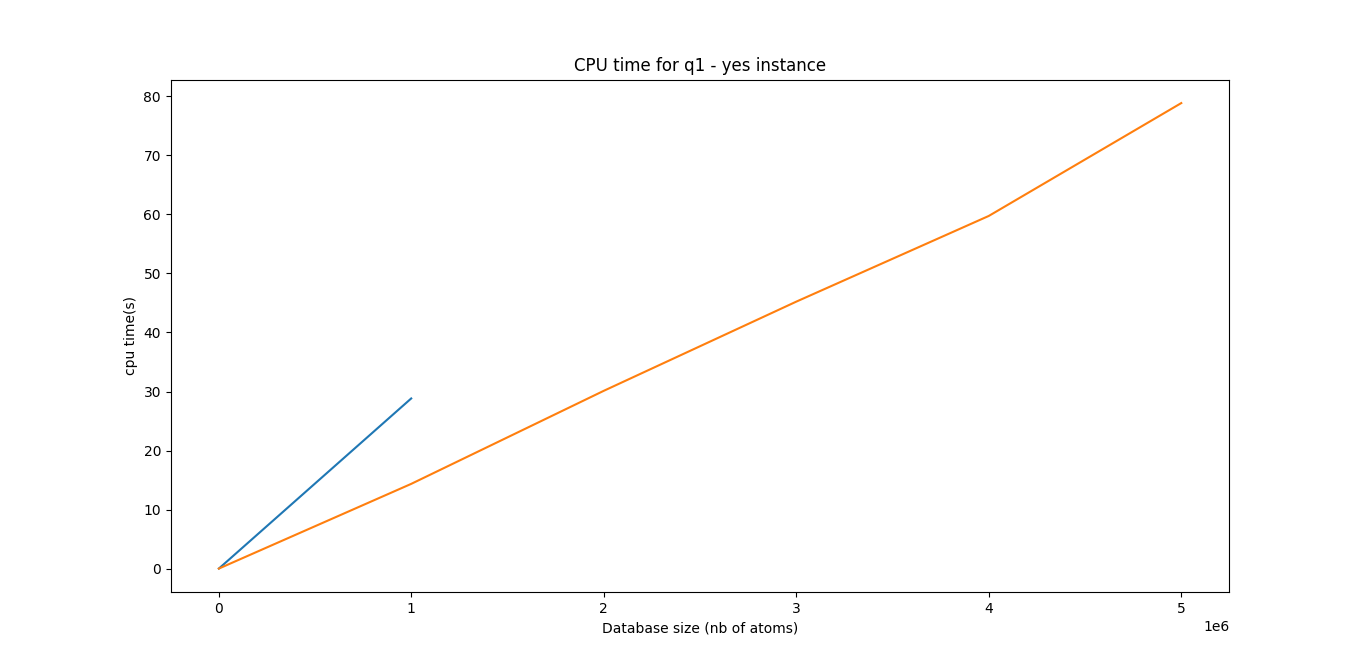
\includegraphics[width=0.6\textwidth]{time_q1_yesinstance.png}
\centering
\end{figure}

\begin{figure}[H]
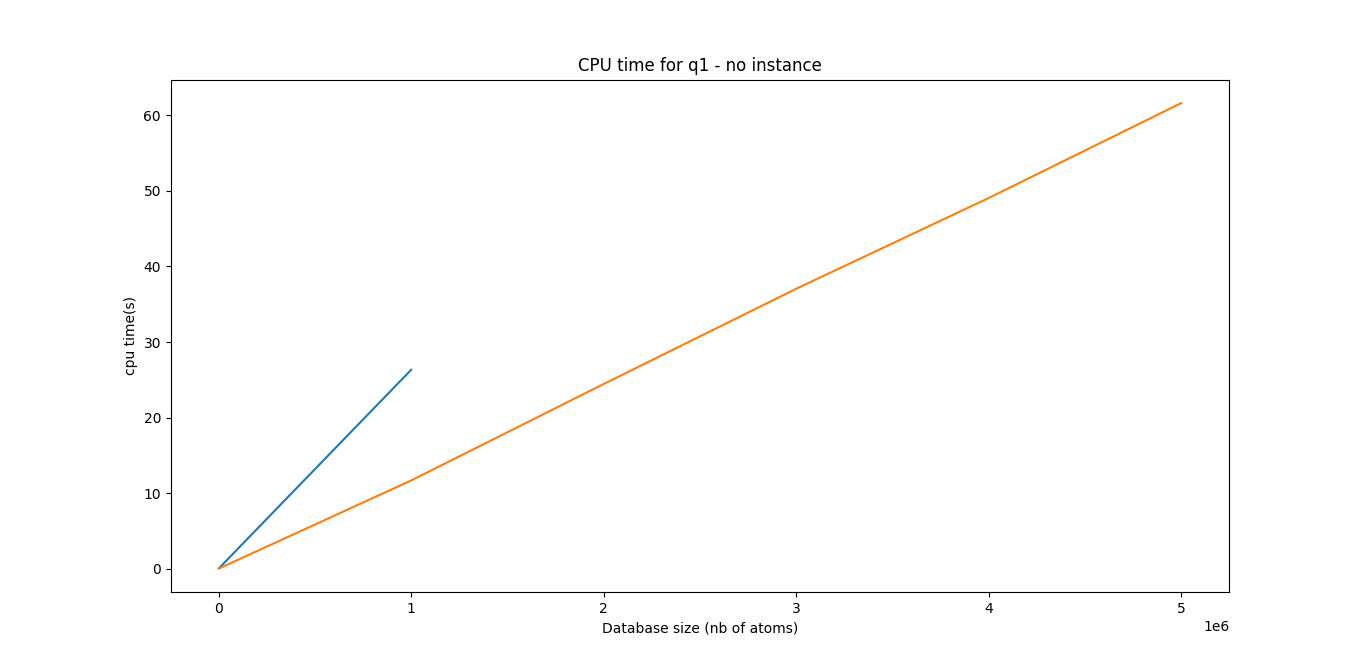
\includegraphics[width=0.6\textwidth]{time_q1_noinstance.png}
\centering
\end{figure}

\begin{figure}[H]
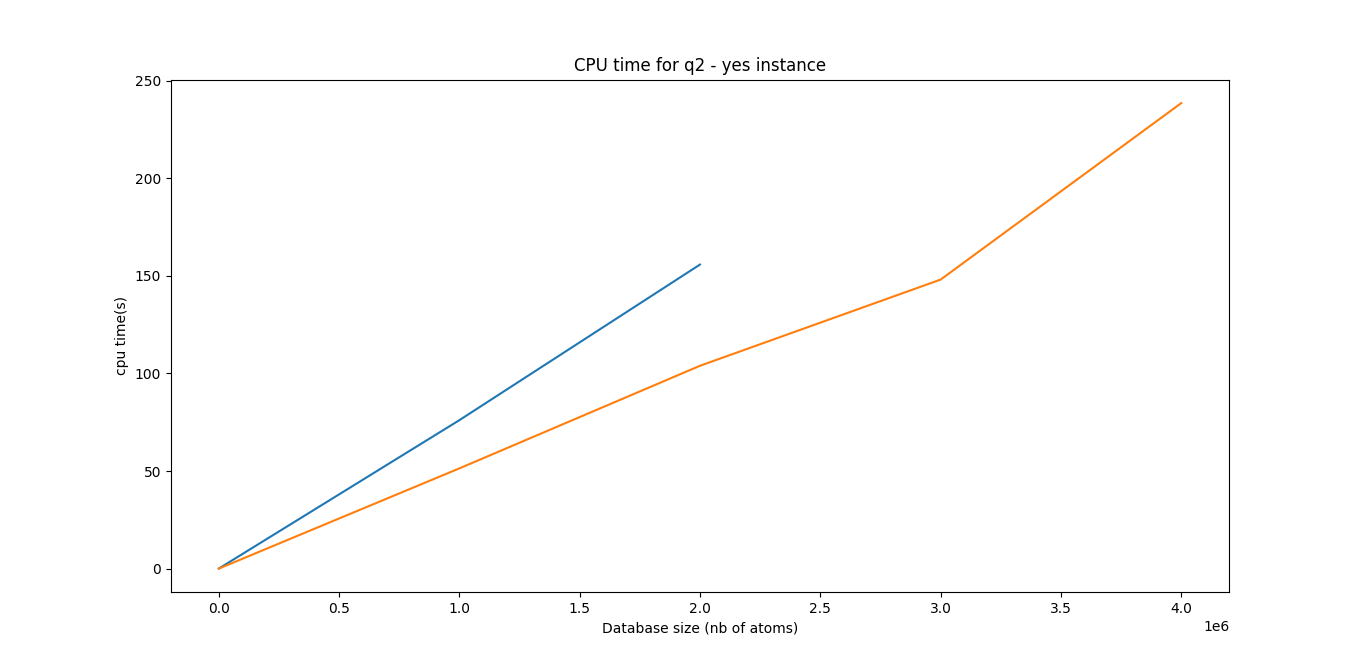
\includegraphics[width=0.6\textwidth]{time_q2_yesinstance.png}
\centering
\end{figure}

\begin{figure}[H]
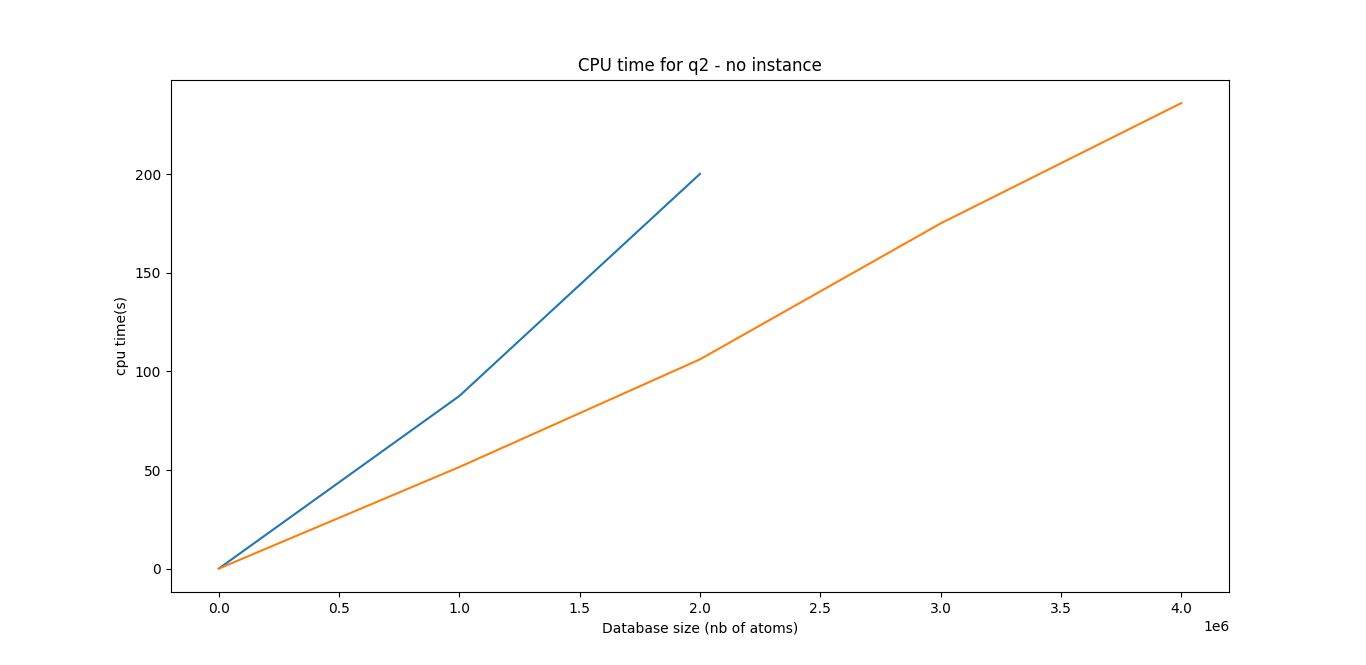
\includegraphics[width=0.6\textwidth]{time_q2_noinstance.png}
\centering
\end{figure}

\begin{figure}[H]
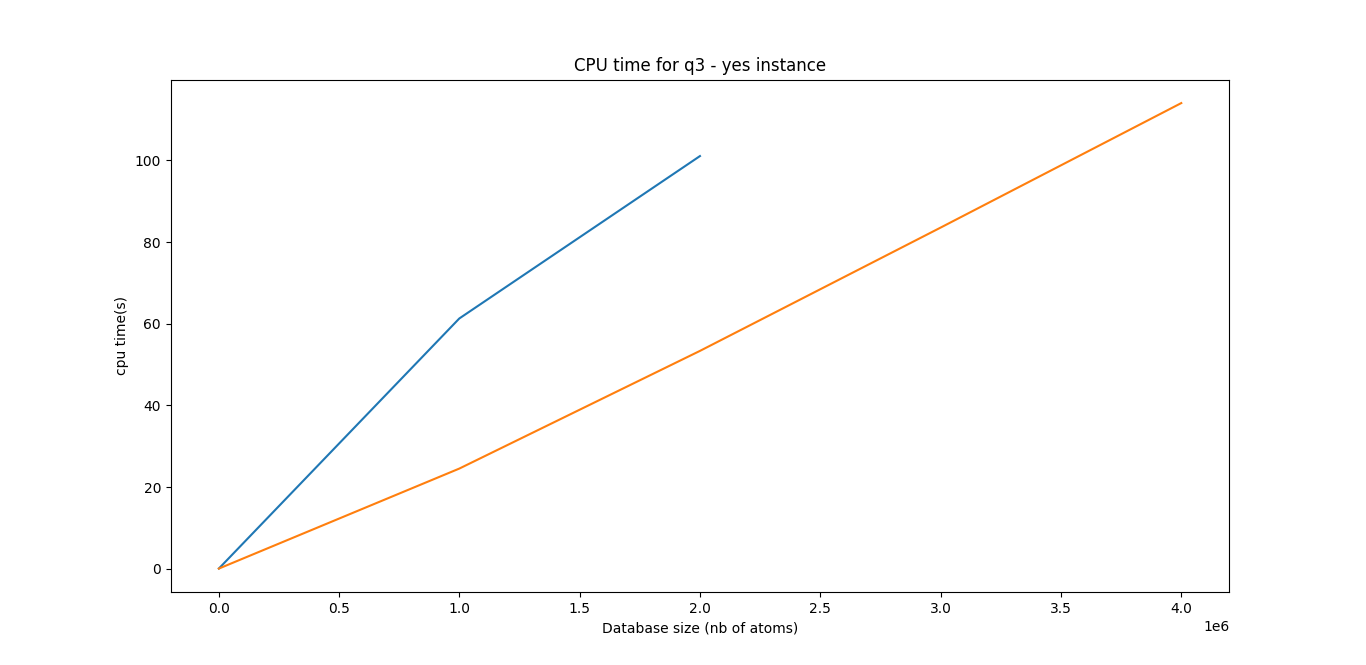
\includegraphics[width=0.6\textwidth]{time_q3_yesinstance.png}
\centering
\end{figure}

\begin{figure}[H]
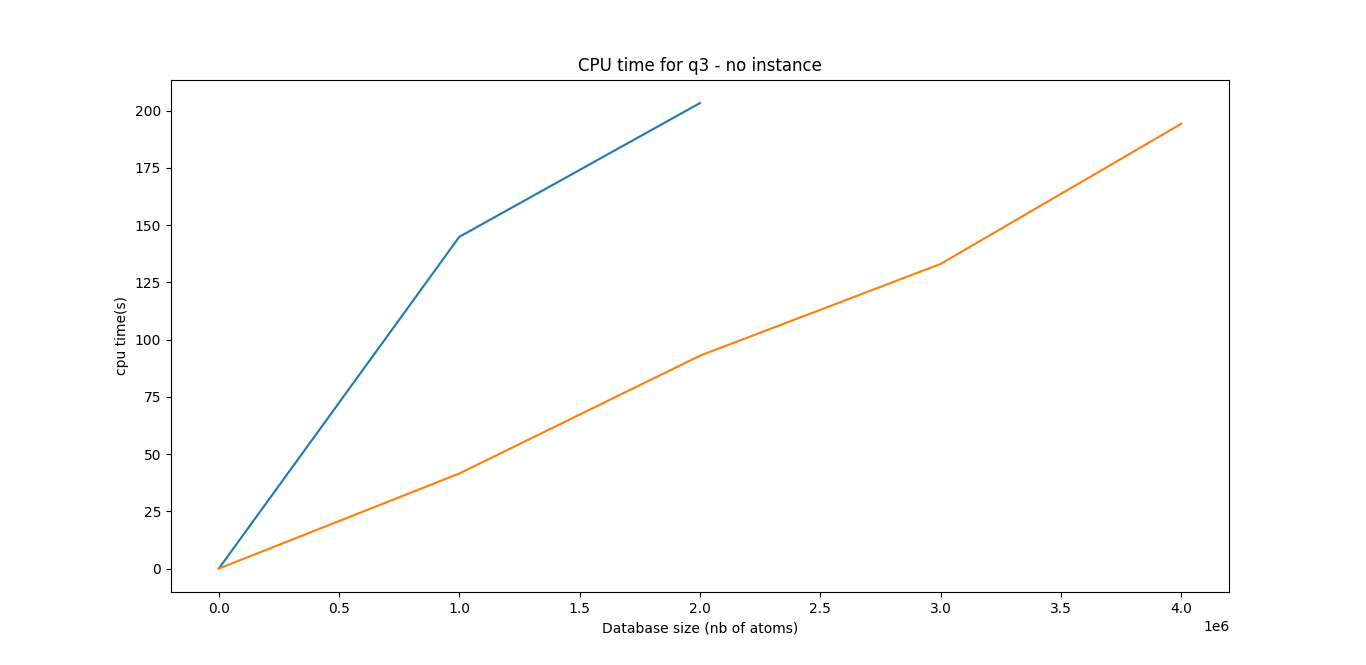
\includegraphics[width=0.6\textwidth]{time_q3_noinstance.png}
\centering
\end{figure}

We see that the fo rewriting leads to better results, in terms of cpu time, that the generate-and-test method.

%%%%%%%%%%%%%%%%%%%%%%%%%%%%%%%%%%%%%%%%%%%%%%%%%%%%%%%%%%%%%%%%%%%%%%%%%%%%%%%%%%%%%%%%%

\section{Conclusion}


We rewrited 7 first-order rewritable queries in ASP and showed that the fo
rewriting are more efficient than a generate and test method. The first order
rewriting consumes a lot less memory than the generate and test which cannot
run on 8GB of RAM on a database containing 3 millions or more entries. Our
experiments show that the first order rewriting is always faster than the
generate in test method wheter the inconsistency is low or high and whether the
database is small or large. We would advice to rewrite any of your queries in
first order if they are rewritable in first order.

\appendix



\end{document}
\endinput

%%
%% End of file `sample-acmsmall-conf.tex'.
